%-----------------------------------------------------------------------------%
\chapter{\babLima}
\label{bab:5}
%-----------------------------------------------------------------------------%

\subsection{OCR Ulang Berkas PDF}\label{ocr-ulang-berkas-pdf}

Dokumen peraturan perundang-undangan yang digunakan pada penelitian
didapatkan dalam format berkas PDF. Penulis pada awalnya mencoba
langsung mengekstraksi data dari PDF, tetapi penulis menemukan
kesulitan. Salahsatu kesulitan yang penulis temui adalah terdapatnya
salah pemindaian pada berkas PDF. Sebagai contoh, terdapat teks yang
tertulis \texttt{Pasal} tetapi mengandung data \texttt{Pasai}. Selain
itu, penulis juga menemukan bahwa setiap dokumen mengandung keslahan
pemindaian yang bervariasi. Untuk suatu kasus, teks \texttt{(2)} selalu
terdeteksi sebagai \texttt{(21} pada suatu dokumen, tetapi tidak pada
dokumen lainnya. Pada kasus lainnya terdapat dokumen yang hampir tidak
memiliki kesalahan pemindaian dan juga terdapat dokumen yang teksnya
tidak dapat dibaca samasekali.

Walaupun dokumen-dokumen tersebut dipelihara oleh satu lembaga pada satu
situs web, yaitu oleh Dewan Perwakilan Rakyat pada situs web
dpr.go.id/jdih, masing-masing dokumen dibuat kedalam berkas PDF dengan
cara yang berbeda-beda. Penulis tidak dapat mengetahui secara pasti
metode apa yang digunakan, tetapi dari metadata yang didapatkan dari
berkas PDF, penulis dapat membuat beberapa dugaan. Pada berkas PDF,
terdapat metadata dengan nama \textbf{Creator}, dimana pada
dokumen-dokumen peraturan Perudang-udangan yang didapatkan, tercantum
nama-nama alat pencetak atau merk dari pencetak tersebut. Dari informasi
tersebut penulis menduga bahwa terdapat sebagian peraturan
perundang-undangan yang dibuat menjadi PDF dengan mencetaknya menjadi
kertas terlebih dahulu kemudian di pindai oleh pemindai dan sebagian
lainnya dikonversi langsung dari berkas \emph{.docx}. Data yang dipindai
adalah berupa gambar, artinya teks yang terdapat pada berkas PDF adalah
hasil OCR (\emph{optical character recognition}) oleh pemindai tersebut.
Berikut adalah salahsatu contoh dokumen beserta data yang tercantum
sebagai \textbf{Creator} dan contoh kesalahan pemindaiannya yang banyak
terjadi.

\begin{longtable}[c]{@{}lll@{}}
\toprule\addlinespace
Dokumen & \textbf{Creator} & Kesalahan pemindaian
\\\addlinespace
\midrule\endhead
UU Nomor 13 Tahun 2003 & ScanSoft PDF Create! 4 & - (tidak ada)
\\\addlinespace
UU Nomor 6 Tahun 2018 & Canon & \texttt{(2)} selalu dipindai
\texttt{(21}
\\\addlinespace
PP Nomor 34 Tahun 2021 & Fuji Xerox B9100 & data teks tidak terbaca
\\\addlinespace
\bottomrule
\end{longtable}

Pemindaian berkas PDF dengan metode yang berbeda-beda memberikan
kualitas hasil pemindaian yang berbeda-beda dan kesalahan pemindaian
yang tidak konsisten. Untuk menyelesaikan masalah ini, penulis melakukan
OCR ulang terhadap semua dokumen yang akan di konversi. Dengan melakukan
OCR ulang menggunakan satu metode yang sama, penulis tidak hanya
berhasil mendapatkan data hasil pemindaian berkas PDF dengan kualitas
pemindaian yang konsisten untuk semua dokumen. Penulis memilih
menggunakan Tesseract OCR
\href{https://github.com/tesseract-ocr/tesseract}{4} sebagai metode OCR
karena sifatnya \emph{open source} dan mendukung Bahasa Indonesia
sebagai bahasa yang dipindai.

Untuk melakukan OCR ulang perlu dilakukan instalasi program yang
dibutuhkan yang dapat dilakukan dengan \emph{command} berikut pada
sistem operasi Ubuntu 20.04. \texttt{ocrmypdf} merupakan \emph{wrapper}
untuk Tesseract OCR dan \texttt{tesseract-ocr-ind} adalah program
tambahan untuk dapat melakukan OCR menjadi teks Bahasa Indonesia.

\begin{Shaded}
\begin{Highlighting}[]
\KeywordTok{sudo} \NormalTok{apt update}
\KeywordTok{sudo} \NormalTok{apt install ocrmypdf tesseract-ocr-ind -y}
\end{Highlighting}
\end{Shaded}

Setelah program diinstall, OCR dapat dilakukan dengan menjalankan
\emph{command} dibawah. Pada contoh dibawah dilakukan konversi
\texttt{UU-2021-34.pdf} yang sudah ada menjadi
\texttt{UU-2021-34\_OCR.pdf} hasil OCR. Opsi \texttt{-{}-force-ocr}
diperlukan untuk melakukan OCR ulang pada berkas PDF yang sudah memiliki
teks hasil OCR untuk di \emph{overwrite}. Opsi \texttt{-{}-jobs 4}
menjalankan \emph{command} dengan 4 \emph{core} CPU, bilangan pada opsi
ini dapat diganti sesuai kebutuhan. Opsi
\texttt{-{}-tesseract-config tesseract-config.cfg} menjalankan
\emph{command} dengan konfigurasi yang diberikan.

\begin{Shaded}
\begin{Highlighting}[]
\KeywordTok{ocrmypdf} \NormalTok{-l ind --force-ocr --jobs 4 --tesseract-config tesseract-config.cfg UU-2021-34.pdf UU-2021-34_OCR.pdf}
\end{Highlighting}
\end{Shaded}

Konfigurasi Tesseract OCR yang digunakan adalah
\texttt{tessedit\_pageseg\_mode 4} seperti yang terlihat pada isi file
konfigurasi dibawah. \texttt{tessedit\_pageseg\_mode 4} digunakan agar
Tesseract OCR mendeteksi teks sebagai \emph{block}, bukan \emph{word}
atau \emph{character}.

\begin{verbatim}
# tesseract-config.cfg
tessedit_pageseg_mode 4
\end{verbatim}

\subsection{Ekstraksi Berkas PDF menjadi Data
\emph{Span}}\label{ekstraksi-berkas-pdf-menjadi-data-span}

\subsubsection{Data \emph{Span}}\label{data-span}

Agar dapat diproses oleh program, berkas PDF perlu diolah menjadi data
berupa daftar teks dan posisinya yang selanjutnya akan disebut
\emph{span}. Sebuah \emph{span} mengandung satu baris teks. Berikut
adalah data yang dimiliki oleh sebuah \emph{span}:

\begin{itemize}
\itemsep1pt\parskip0pt\parsep0pt
\item
  \texttt{str}: teks yand dikandung
\item
  \texttt{xL}: koordinat titik terkiri dari \emph{span}
\item
  \texttt{xR}: koordinat titik terkanan dari \emph{span}
\item
  \texttt{y}: koordinat titik teratas dari \emph{span}
\item
  \texttt{pageNum}: nomor halaman
\item
  \texttt{id}: \emph{identifier} unik untuk setiap span
\end{itemize}

Berikut adalah contoh gambaran berkas PDF dan hasil ekstraksinya menjadi
daftar \emph{span}.

\begin{figure}[htbp]
\centering
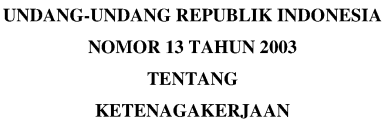
\includegraphics{pictures/pdf_example.png}
\caption{Gambar berkas PDF yang akan diekstraksi}
\end{figure}

akan dipindai menjadi

\begin{Shaded}
\begin{Highlighting}[]
\KeywordTok{-} \FunctionTok{xL:} \NormalTok{197.52}
  \FunctionTok{xR:} \NormalTok{442.79990000000004}
  \FunctionTok{'y':} \NormalTok{234.48000000000002}
  \FunctionTok{str:} \NormalTok{UNDANG-UNDANG REPUBLIK INDONESIA}
  \FunctionTok{pageNum:} \NormalTok{1}
  \FunctionTok{id:} \NormalTok{0}
\KeywordTok{-} \FunctionTok{xL:} \NormalTok{252.72}
  \FunctionTok{xR:} \NormalTok{387.6002}
  \FunctionTok{'y':} \NormalTok{255.12}
  \FunctionTok{str:} \NormalTok{NOMOR 13 TAHUN 2003}
  \FunctionTok{pageNum:} \NormalTok{1}
  \FunctionTok{id:} \NormalTok{1}
\KeywordTok{-} \FunctionTok{xL:} \NormalTok{291.12}
  \FunctionTok{xR:} \NormalTok{349.68048}
  \FunctionTok{'y':} \NormalTok{275.76}
  \FunctionTok{str:} \NormalTok{TENTANG}
  \FunctionTok{pageNum:} \NormalTok{1}
  \FunctionTok{id:} \NormalTok{2}
\KeywordTok{-} \FunctionTok{xL:} \NormalTok{257.28}
  \FunctionTok{xR:} \NormalTok{383.28015999999997}
  \FunctionTok{'y':} \NormalTok{296.4}
  \FunctionTok{str:} \NormalTok{KETENAGAKERJAAN}
  \FunctionTok{pageNum:} \NormalTok{1}
  \FunctionTok{id:} \NormalTok{3}
\end{Highlighting}
\end{Shaded}

\subsubsection{Membersihkan \emph{Noise} dari
Halaman}\label{membersihkan-noise-dari-halaman}

Tidak jarang dokumen peraturan Perudang-undangan mengandung data
\emph{noise} yang tidak ingin kita ekstraksi seperti \emph{header} dan
\emph{footer}. Pada penelitian ini, penulis menggunakan dokumen dari
sumber yang sama sehingga memiliki format yang sama, dan juga posisi
\emph{header} dan \emph{footer} yang hampir sama pada setiap dokumen.

\begin{figure}[htbp]
\centering

\includegraphics{pictures/pdf_header.png}
\caption{Contoh Header}
\end{figure}

Gambar diatas adalah contoh \emph{header} yang terdapat pada setiap
halaman. Dapat dilihat bahwa \emph{header} selalu terdiri dari teks
``PRESIDEN REPUBLIK INDONESIA'' dan diikuti oleh nomor halaman, dan
selalu terletak di posisi yang hampir sama. Oleh karena itu, penulis
memeriksa teks menggunakan \emph{regex} dan posisi dari setiap
\emph{span}, kemudian menghapus \emph{span} tersebut jika terdeteksi
sebagai header.

\subsubsection{Penggabungan Data Berkas PDF Asli dan Hasil OCR
Ulang}\label{penggabungan-data-berkas-pdf-asli-dan-hasil-ocr-ulang}

Pada proses ekstraksi berkas PDF menjadi daftar \emph{span}, penulis
menemukan satu masalah yaitu data hasil OCR tidak konsisten dalam
memindai angka. Seperti yang dapat dilihat pada gambar dibawah, angka 10
berhasil dipindai tetapi angka 9 tidak berhasil. Untuk kasus dibawah,
angka hanya tidak terpindai pada hasil OCR ulang, tetapi terpindai
dengan benar pada berkas PDF aslinya. Untuk menyelesaikan masalah
tersebut, penulis melakukan ekstraksi data pada berkas PDF aslinya,
kemudian menggabungkannya dengan data hasil pemindaian untuk melengkapi
bagian yang tidak terpindai.

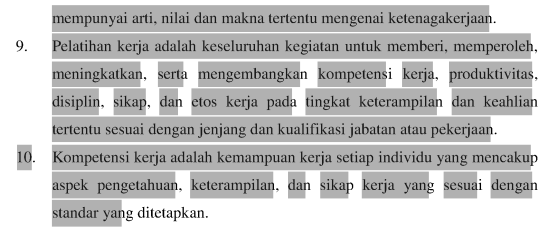
\includegraphics{pictures/pdf_unscanned_number.png})

Penulis hanya menggabungkan data dua berkas PDF untuk kasus angka
seperti yang disebutkan diatas. Hal tersebut dikarenakan pada umumnya
kita dapat mentolerir kesalahan pemindaian pada teks, tetapi karena
kegagalan pemindaian pada angka tersebut akan mempengaruhi struktur
dokumen, penulis memutuskan solusi diatas. Sebagai contoh, jika nomor 8
berhasil dipindai dan nomor 9 tidak berhasil, maka struktur akhir yang
dihasilkan akan mengandung semua isi nomor 9 didalam nomor 8, yang mana
seharusnya adalah nomor yang terpisah. Berikut berturut-turut adalah
contoh data yang dihasilkan jika nomor 9 tidak berhasil terpindai dan
jika berhasil terpindai.

Jika nomor 9 tidak berhasil terpindai:

\begin{Shaded}
\begin{Highlighting}[]
\KeywordTok{-} \FunctionTok{type:} \NormalTok{point}
  \FunctionTok{key:} \NormalTok{8}
  \FunctionTok{text:} \NormalTok{>-}
    \NormalTok{Informasi ketenagakerjaan adalah gabungan, rangkaian, dan analisis data yang}
    \NormalTok{berbentuk angka yang telah diolah, naskah dan dokumen yang mempunyai arti,}
    \NormalTok{nilai dan makna tertentu mengenai ketenagakerjaan.}
    \NormalTok{9. Pelatihan kerja adalah keseluruhan kegiatan untuk memberi, memperoleh,}
    \NormalTok{meningkatkan, serta mengembangkan kompetensi kerja, produktivitas, disiplin,}
    \NormalTok{sikap, dan etos kerja pada tingkat keterampilan dan keahlian tertentu sesuai}
    \NormalTok{dengan jenjang dan kualifikasi jabatan atau pekerjaan.}
\end{Highlighting}
\end{Shaded}

Jika nomor 9 berhasil terpindai:

\begin{Shaded}
\begin{Highlighting}[]
\KeywordTok{-} \FunctionTok{type:} \NormalTok{point}
  \FunctionTok{key:} \NormalTok{8}
  \FunctionTok{text:} \NormalTok{>-}
    \NormalTok{Informasi ketenagakerjaan adalah gabungan, rangkaian, dan analisis data yang}
    \NormalTok{berbentuk angka yang telah diolah, naskah dan dokumen yang mempunyai arti,}
    \NormalTok{nilai dan makna tertentu mengenai ketenagakerjaan.}
\KeywordTok{-} \FunctionTok{type:} \NormalTok{point}
  \FunctionTok{key:} \NormalTok{9}
  \FunctionTok{text:} \NormalTok{>-}
    \NormalTok{Pelatihan kerja adalah keseluruhan kegiatan untuk memberi, memperoleh,}
    \NormalTok{meningkatkan, serta mengembangkan kompetensi kerja, produktivitas, disiplin,}
    \NormalTok{sikap, dan etos kerja pada tingkat keterampilan dan keahlian tertentu sesuai}
    \NormalTok{dengan jenjang dan kualifikasi jabatan atau pekerjaan.}
\end{Highlighting}
\end{Shaded}

\subsection{Klasifikasi Dokumen}\label{klasifikasi-dokumen}

Pa

\subsection{Pengelompokan \emph{span} menjadi
Komponen}\label{pengelompokan-span-menjadi-komponen}

Teks yang membentuk suatu komponen terdiri dari satu atau lebih
\emph{span}, sehingga daftar \emph{span} yang didapatkan dari hasil
ekstraksi berkas PDF harus dikelompokkan sehingga setiap kelompok
merepresentasikan \emph{span} yang terdapat pada suatu komponen.
Pengelompokan dilakukan dengan mendeteksi \emph{span} awal dan
\emph{span} akhir dari sebuah komponen. Karena daftar \emph{span} hasil
ekstraksi bersifat 1 dimensi, hal ini bisa dilakukan dengan melakukan
iterasi pada setiap \emph{span}, kemudian menandai awal atau akhir dari
sebuah kelompok apabila memenuhi suatu pola. Setelah ditandai,
\emph{span} akan dikelompokkan sebagai daftar \emph{span} dari suatu
komponen.

Pengelompokan tidak langsund dilakukan dari daftar \emph{list} menjadi
daftar komponen, melainkan dibuat pengelompokan \emph{section} untuk
pembagian dokumen secara garis besar, kemudian baru dikelompokkan
sebagai komponen dari masing-masing \emph{section} tersebut. Pada gambar
dibawah \emph{section} ditandai dengan warna biru dan komponen ditandai
dengan warna merah. Dapat dilihat bahwa daftar \emph{span} data awal
dikelompokkan menjadi beberapa \emph{section} yaitu \texttt{judul},
\texttt{metadata}, \texttt{babset}, dan \texttt{disahkan}. Kemudian
\emph{span} pada section \texttt{babset} dikelompokkan menjadi komponen
bab yaitu \texttt{Bab 1}, \texttt{Bab 2}, dan \texttt{Bab 3}. Kemudian
\emph{span} pada setiap komponen bab dikelompokkan menjadi komponen
pasal. Pengelompokan bertingkat ini dilakukan agar fungsi untuk
mendeteksi batas antara komponen tidak menjadi rumit.

\begin{figure}[htbp]
\centering

\includegraphics{pictures/pdf_to_component.svg}
\caption{Ilustrasi Ekstraksi Daftar Span menjadi Data Struktur Komponen}
\end{figure}

Deteksi batas antara komponen atau \emph{section} dilakukan dengan
melihat data pada \emph{span} seperti \texttt{str}, \texttt{xL},
\texttt{xR}, dan \texttt{y}. Pada gambar diatas, pola yang terdeteksi
sebagai batas ditandai dengan huruf merah. Sebagai contoh, pada ekstraki
paling kiri, dari daftar \emph{span} asli menjadi \emph{section},
dilakukan iterasi \emph{span} dari atas dan akan dimasukkan ke dalam
\emph{section} \texttt{judul} sampai menemukan \emph{section} yang
diawali dengan kata \textbf{Menimbang}. Kemudian setiap \emph{span}
setelah span \textbf{Menimbang} tersebut akan dikelompokkan menjadi
\emph{section} \texttt{metadata} sampai menemukan section yang diawali
kata \textbf{BAB I}.

\subsubsection{Pengelompokan \emph{span} pada Komponen
Terurut}\label{pengelompokan-span-pada-komponen-terurut}

Beberapa komponen seperti \texttt{bab}, \texttt{bagian},
\texttt{paragraf}, \texttt{pasal}, \texttt{angka}, dan \texttt{huruf}
memiliki sifat terurut. Dalam hal ini, yang termasuk terurut adalah:

\begin{itemize}
\itemsep1pt\parskip0pt\parsep0pt
\item
  Komponen yang mengawali suatu komponen terurut akan selalu sama.
\item
  Hanya terdapat satu komponen yang dapat mengikuti komponen terurut.
\end{itemize}

Contoh dari sifat pertama adalah \texttt{bab}, \texttt{bagian},
\texttt{paragraf}, \texttt{pasal}, \texttt{angka} pasti dimulai dari
komponen nomor 1 seperti \texttt{bab 1} dan \texttt{pasal 1}, dan
\texttt{huruf} pasti dimulai dari komponen \texttt{huruf a}. Contoh dari
sifat kedua adalah hanya \texttt{pasal 2} yang dapat mengikuti
\texttt{pasal 1} dan hanya \texttt{huruf b} yang dapat mengikuti
\texttt{huruf a}. Dalam implementasi, penulis memastikan sifat-sifat ini
dipatuhi, sehingga sebagai contoh apabila sebuah dokumen terdeteksi
mengandung \texttt{bab 12} maka akan dijamin mengandung semua
\texttt{bab 1} sampai \texttt{bab 11} dan apabila terdeteksi mengandung
\texttt{pasal 196} maka akan dijamin mengandung semua pasal dari
\texttt{pasal 1} sampai \texttt{pasal 195}.

\subsubsection{Komponen Amandemen}\label{komponen-amandemen}

Mengekstraksi \emph{span} pada bagian amandemen merupakan salahsatu
tantangan pada penelitian ini. Dibawah adalah gambar amandemen pada
Pasal 17 UU Nomor 11 Tahun 2020 yang dilakukan terhadap Pasal 1 UU Nomor
26 Tahun 2007. Dapat dilihat bahwa kata \texttt{Pasal 17} dan
\texttt{Pasal 1} yang digunakan sebagai pembatas antara komponen
memiliki pola teks dan posisi yang hampir sama. Hal ini membuat
pembedaan antara ``Pasal biasa'' dan ``Pasal peng-amandemen'' menjadi
sulit dilakukan.

\begin{figure}[htbp]
\centering
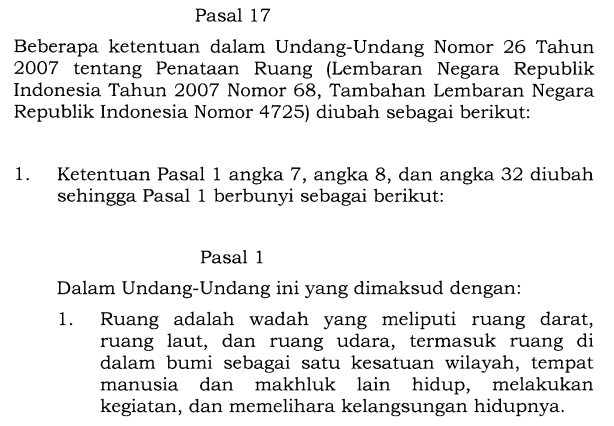
\includegraphics{pictures/pdf_amendment.png}
\caption{Contoh Amendemen pada UU Nomor 11 Tahun 2020}
\end{figure}

Untuk menyelesaikan masalah ini, penulis menggunakan koordinat
\texttt{xL} \emph{span} tepat setelah \emph{span} yang bertuliskan
``Pasal X''. Pada contoh deteksi kompoonen amandemen di bawah,
\texttt{xL} dari teks setelah pasal peng-amandemen (pasal biasa)
ditandai dengan lingkaran merah, \texttt{xL} dari pasal yang diamandemen
ditandai dengan lingkaran biru, dan garis hijau merepresentasikan batas
pemeda \texttt{xL} antara pasal biasa dan pasal yang diamandemen.
Pembedaan pasal biasa dan pasal amandemen hanya dilakukan jika dokumen
memiliki komponen berupa amandemen.

\begin{figure}[htbp]
\centering

\includegraphics{pictures/amendment_detection.svg}
\caption{Deteksi Komponen Amandemen}
\end{figure}

\subsection{Deteksi Sitasi}\label{deteksi-sitasi}

Setelah semua \emph{span} dikelompokan menjadi suatu komponen, dilakukan
deteksi sitasi pada teks pada setiap komponen untuk mengetahui apakah
komponen tersebut menyebut komponen atau dokumen peraturan
perundang-undangan lainnya. Berikut adalah daftar pola sitasi yang
berhasil dideteksi pada penelitian ini.

\begin{longtable}[c]{@{}lll@{}}
\toprule\addlinespace
Pola & Contoh teks & URI Terdeteksi
\\\addlinespace
\midrule\endhead
Undang Undang Dasar Negara Republik Indonesia Tahun 1945 & Undang Undang
Dasar Negara Republik Indonesia Tahun 1945 & /uud/
\\\addlinespace
Undang-Undang Nomor \{x\} Tahun \{y\} & Undang-Undang Nomor 26 Tahun
2007 & /uu/2007/26
\\\addlinespace
ayat (\{x\}) & ayat (1) & /uu/2003/13/pasal/169/ayat/1
\\\addlinespace
Pasal \{x\} & Pasal 156 & /uu/2003/13/pasal/156
\\\addlinespace
Pasal \{x\} ayat (\{y\}) & Pasal 156 ayat (2) &
/uu/2003/13/pasal/156/ayat/2
\\\addlinespace
huruf \{x\}, \{y\}, \ldots{} dan \{z\} & huruf a, b, c, d, dan e &
/uu/2003/13/menimbang/point/a
\\\addlinespace
& & /uu/2003/13/menimbang/point/b
\\\addlinespace
& & /uu/2003/13/menimbang/point/c
\\\addlinespace
& & /uu/2003/13/menimbang/point/d
\\\addlinespace
& & /uu/2003/13/menimbang/point/e
\\\addlinespace
huruf \{x\} dan \{y\} & huruf a dan b &
/uu/2003/13/pasal/1/point/5/point/a
\\\addlinespace
& & /uu/2003/13/pasal/1/point/5/point/b
\\\addlinespace
\bottomrule
\end{longtable}

Data sitasi mengandung data sebagai berikut:

\begin{itemize}
\itemsep1pt\parskip0pt\parsep0pt
\item
  \texttt{start}: \emph{index} karakter awal sitasi
\item
  \texttt{end}: \emph{index} karakter akhir sitasi
\item
  \texttt{uri}: URI dokumen dan
\end{itemize}

Berikut adalah contoh teks pada Undang-Undang Nomor 13 Tahun 2003 Pasal
158 Ayat (4) beserta sitasi yang terdeteksi.

\begin{Shaded}
\begin{Highlighting}[]
\FunctionTok{textString:} \NormalTok{>-}
  \NormalTok{Pekerja/buruh yang diputus hubungan kerjanya berdasarkan alasan sebagaimana}
  \NormalTok{dimaksud dalam ayat (1), dapat memperoleh uang penggantian hak sebagaimana}
  \NormalTok{dimaksud dalam Pasal 156 ayat (4).}
\FunctionTok{references:}
  \KeywordTok{-} \FunctionTok{start:} \NormalTok{91}
    \FunctionTok{end:} \NormalTok{99}
    \FunctionTok{uri:} \NormalTok{/uu/2003/13/pasal/158/ayat/1}
  \KeywordTok{-} \FunctionTok{start:} \NormalTok{166}
    \FunctionTok{end:} \NormalTok{184}
    \FunctionTok{uri:} \NormalTok{/uu/2003/13/pasal/156/ayat/4}
\end{Highlighting}
\end{Shaded}

Untuk melakukan deteksi, teks akan melalui fungsi yang masing-masing
memiliki pola untuk dideteksi. Oleh karena itu, untuk \emph{substring}
yang beririsan dapat memiliki lebih dari dua sitasi yang terdeteksi.
Pada kasus tersebut akan diambil sitasi dengan \emph{substring}
terpanjang. Sebagai contoh, teks ``Pasal 156 Ayat (4)'' pada UU No.13
Tahun 2003 Pasal 158 Ayat (4) akan terdeteksi sebagai 3 URI sitasi
sebagai berikut.

\begin{longtable}[c]{@{}ll@{}}
\toprule\addlinespace
Teks & URI
\\\addlinespace
\midrule\endhead
Pasal 156 Ayat (4) & \texttt{/uu/2003/13/pasal/156/ayat/4}
\\\addlinespace
Pasal 156 & \texttt{/uu/2003/13/pasal/156}
\\\addlinespace
Ayat (4) & \texttt{/uu/2003/13/pasal/158/ayat/4}
\\\addlinespace
\bottomrule
\end{longtable}

Pada kasus ini, yang akan diambil adalah teks ``Pasal 156 ayat (4)''
karena merupakan teks terpanjang.

\subsection{Data To MD}\label{data-to-md}

visualization

\subsection{Data to triple}\label{data-to-triple}

\subsubsection{triple definition}\label{triple-definition}

\subsubsection{triple to ttl}\label{triple-to-ttl}

\subsection{Query}\label{query}

Fuseki

\section{BAB 5 EVALUASI DAN ANALISIS
HASIL}\label{bab-5-evaluasi-dan-analisis-hasil}

\subsection{Aplikasi Knowledge Graph Peraturan
Perundang-undangan}\label{aplikasi-knowledge-graph-peraturan-perundang-undangan}

Dibuat \emph{chatbot} untuk mensimulasikan pengaplikasian KG.
\emph{Chatbot} akan memproses input yand diberikan oleh user, kemudian
meng-\emph{generate} SPARQL \emph{query}. Chatbot akan menampilkan hasil
dari \emph{query} tersebut.

\subsection{Evaluasi Hasil Konversi}\label{evaluasi-hasil-konversi}

Evaluasi akan dilakukan terhadap semua dokumen yang terdapat pada
peraturan.go.id. Selanjutnya dokumen-dokumen ini akan disebut dokument
tes.

\subsection{Evaluasi Manual}\label{evaluasi-manual}

Evaluasi kualitatif dilakukan terhadap sebagian dokumen yang didapatkan
dari hasil sam- pling dari dokumen tes. Seorang penilai akan melihat
markdown dari setiap dokumen hasil sampling, masing-masing dokumen akan
diberikan skor 0 sampai 100. Kualitas konversi dapat dilihat dari
rata-rata skor tersebut.

\subsection{Evaluasi Otomatis}\label{evaluasi-otomatis}

Evaluasi dilakukan dengan terlebih dahulu mendefinisikan metadata yang
pasti terdapat pada sebuah dokumen (misal, tempat dokumen disahkan),
kemudian menghitung sebera pa banyak metadata yang berhasil diekstrak.
Metadata hasil ekstraksi yang akan dihitung tidak perlu sesuai dengan
yang terdapat di dalam dokumen.

{[}6{]}:
\url{https://op.europa.eu/en/publication-detail/-/publication/514875b4-5efd-11e8-ab9c-01aa75ed71a}
1


